\section{Giới thiệu}

Bài toán logic puzzle là một môi trường phù hợp để nghiên cứu tìm kiếm trong
Trí tuệ nhân tạo: luật chơi xác định rõ tập trạng thái, các hành động và điều
kiện thành công. Trong báo cáo này, đối tượng nghiên cứu là \textbf{Pipes}, một
trò chơi xoay các đoạn ống để tạo thành một mạng liên thông không có chu trình.
Hai chiến lược được hiện thực bằng Python 3 là \textbf{Depth-First Search (DFS)}
và \textbf{Greedy Best-First Search (GBFS)}. Các khái niệm tìm kiếm và ràng buộc
được sử dụng theo cách trình bày trong tài liệu \emph{Artificial Intelligence:
A Modern Approach}, Chương 3 và Chương 6~\cite{aima}.

Nội dung tập trung vào việc mô hình hóa Pipes, xây dựng bộ sinh trạng thái kế
tiếp, giải thích thuật toán và so sánh thời gian thực thi cùng bộ nhớ đỉnh trên
các đầu vào giống nhau. Chương trình có giao diện Pygame để minh họa từng bước
mở rộng, thử hướng ống, loại nhánh và quay lui. Phạm vi đánh giá là tìm
\emph{một cấu hình hợp lệ}; chương trình không tối ưu số lần người chơi phải
nhấp chuột để xoay ống. Phạm vi báo cáo là bài toán Pipes.

\section{Bài toán Pipes}
\subsection{Luật chơi và mục tiêu}

Pipes sử dụng một lưới vuông gồm các ô chứa đoạn ống. Người chơi xoay từng ô
theo góc $90^\circ$ để nối toàn bộ đường ống thành một nhóm; luật gốc không cho
phép chu trình kín~\cite{pipes}. Phiên bản hiện thực hỗ trợ kích thước
$4\times4$, $5\times5$ và $7\times7$, với biên thông thường, không nối vòng
từ cạnh này sang cạnh đối diện. Một lời giải phải đồng thời thỏa mãn:
\begin{enumerate}
\item Không có đầu ống hướng ra ngoài lưới.
\item Hai ô kề nhau phải khớp đầu ống: có cổng Đông thì ô bên phải có cổng Tây,
      và ngược lại. Hai phía không có cổng cũng phải nhất quán.
\item Tất cả các ô thuộc cùng một thành phần liên thông.
\item Mạng kết nối không chứa chu trình.
\end{enumerate}

\begin{figure}[H]
\centering
\begin{subfigure}{.43\textwidth}\centering
\begin{tikzpicture}[scale=.76]
\pipeboard{2,9,1,6,4,5,1,10,14,13,15,7,6,4,2,4}{muted}
\end{tikzpicture}\caption{Cấu hình đầu vào.}\end{subfigure}
\hspace{8mm}
\begin{subfigure}{.43\textwidth}\centering
\begin{tikzpicture}[scale=.76]
\pipeboard{2,12,2,12,4,5,4,5,7,11,15,13,3,8,1,1}{water}
\end{tikzpicture}\caption{Một lời giải hợp lệ do DFS tìm được.}\end{subfigure}
\caption{Đầu vào \code{pipes-4x4-261.json} và kết quả giải. Chấm xanh là ô nguồn.}
\label{fig:board}
\end{figure}

Ô nguồn nước chỉ là điểm bắt đầu cho việc hiển thị liên thông. Khi toàn bộ
mạng đã liên thông, chọn bất kỳ ô nào làm nguồn đều đi tới mọi ô còn lại.
Do đó, thay đổi nguồn không thay đổi tập cấu hình đích hợp lệ.

\subsection{Định nghĩa trạng thái và bước chuyển hợp lệ}
\subsubsection{Biểu diễn đầu vào}

Gọi kích thước cạnh là $m$ và tổng số ô là $n=m^2$. Đánh số ô từ $0$ đến
$n-1$ theo thứ tự từ trái sang phải, từ trên xuống dưới. Mỗi hướng ống là tập
các cổng trong $\{N,E,S,W\}$. Mã nguồn biểu diễn bằng mặt nạ bit:
$N=1$, $E=2$, $S=4$, $W=8$. Ví dụ, \code{NS} là ống thẳng,
\code{NE} là ống góc và \code{NESW} là ngã tư.

Các bản đồ được lưu bằng JSON; tên tệp là mã định danh đầu vào. Bản đồ không
lưu lời giải, mã phiên bản, ID trùng lặp hay seed sinh ngẫu nhiên:
\begin{lstlisting}[numbers=none,basicstyle=\ttfamily\footnotesize]
{
  "size": 4,
  "source": [2, 2],
  "tiles": [
    ["E", "NW", "N", "ES"],
    ["S", "NS", "N", "EW"],
    ["ESW", "NSW", "NESW", "NES"],
    ["ES", "S", "E", "S"]
  ]
}
\end{lstlisting}

Tọa độ \code{source} có dạng [hàng, cột], bắt đầu từ 0. Vì vậy [2,2] là
hàng thứ ba, cột thứ ba. Dữ liệu lưới là đầu vào thực tế của cả hai thuật toán.
Bộ nạp kiểm tra kích thước, số hàng/cột, các ký tự cổng và tọa độ nguồn.

\subsubsection{Trạng thái tìm kiếm}

Với ô $i$, ký hiệu $\R_i$ là tập các hướng xoay \emph{khác nhau} của hình ống.
Trạng thái tìm kiếm là một tiền tố:
\begin{equation}
s=(a_0,a_1,\ldots,a_{k-1}),\qquad a_i\in\R_i,\quad 0\leq k\leq n.
\label{eq:state}
\end{equation}
Các ô $0,\ldots,k-1$ đã được gán hướng; những ô còn lại chưa được quyết định.
Trạng thái đầu là tiền tố rỗng $s_0=()$, dù chương trình đã biết hình dạng của
toàn bộ ô từ tệp đầu vào. Giao diện vẫn vẽ hướng ban đầu cho những ô chưa gán
để người xem nhận biết hình dạng của chúng.

\begin{table}[H]\centering\small
\begin{tabularx}{\textwidth}{@{}p{.25\textwidth}X@{}}\toprule
Thành phần & Định nghĩa \\\midrule
Trạng thái đầu & Tiền tố rỗng, với toàn bộ hình dạng ô đã biết.\\
Hành động & Chọn một hướng cho ô thứ $k=|s|$.\\
Hàm chuyển & $s'=s+(a_k)$, nếu vượt qua các kiểm tra khả thi.\\
Trạng thái đích & Gán đủ $n$ ô và mạng ống thỏa mãn mọi luật.\\
Chi phí bước & Có thể quy ước 1 cho một phép gán; hai thuật toán không xếp hạng theo chi phí này.\\
Thứ tự biến & Cố định theo hàng, không chọn ô bằng MRV.\\\bottomrule
\end{tabularx}
\caption{Mô hình tìm kiếm dùng chung cho DFS và GBFS.}\label{tab:model}
\end{table}

\subsubsection{Sinh bước chuyển và kiểm tra đích}

Tại độ sâu $k$, thuật toán thử các hướng còn lại của ô $k$. Các phép xoay tạo
ra cùng hình dạng được loại trùng. Hướng ống vượt biên được bỏ trước khi duyệt.
Trạng thái con chỉ được chấp nhận khi vượt qua các điều kiện ở
Mục~\ref{sec:pruning}. Ví dụ, một ống góc tại góc trên trái chỉ có thể mở về
Đông và Nam. Khi ô bên trái đã mở cổng Đông, ô đang xét phải có cổng Tây.

Một bước gán của bộ giải khác một lần nhấp chuột trong trò chơi. Gán hướng
tuyệt đối có thể tương ứng với 0, 1, 2 hoặc 3 lần xoay thuận chiều kim đồng hồ.
Sự kiện loại nhánh hay quay lui là sự kiện tìm kiếm, không phải một lần xoay
vật lý bổ sung. Vì cả DFS và GBFS cùng sử dụng mô hình này, số trạng thái mở
rộng có cùng ý nghĩa khi so sánh hai phương pháp.

Hàm \code{validate_solution()} xác nhận hướng của từng ô vẫn thuộc tập xoay
của hình gốc, sau đó kiểm tra mạng hoàn chỉnh bằng \code{inspect_board()}.
Mỗi ô là một đỉnh; mỗi cặp cổng khớp nhau là một cạnh vô hướng. Một phép duyệt
đồ thị từ nguồn kiểm tra liên thông; phép duyệt có theo dõi đỉnh cha kiểm tra
chu trình. Thuật toán chấp nhận bất kỳ lời giải hợp lệ nào, không so sánh với
một đáp án ẩn của bộ sinh.

\subsection{Không gian tìm kiếm}

Số hướng phân biệt phụ thuộc đối xứng của hình ống:
\begin{table}[H]\centering
\begin{tabular}{@{}lc@{}}\toprule
Loại ống & Số hướng phân biệt $r_i=|\R_i|$\\\midrule
Đầu ống, ống góc, ngã ba & 4\\
Ống thẳng & 2\\
Ngã tư & 1\\\bottomrule
\end{tabular}
\caption{Loại các phép xoay trùng nhau trước khi tìm kiếm.}
\end{table}

Trước khi xét biên và ràng buộc, số cấu hình đầy đủ là:
\begin{equation}
U=\prod_{i=0}^{n-1}r_i\leq4^n.
\end{equation}
Cây tiền tố có độ sâu tối đa $n$, hệ số phân nhánh không quá 4. Tổng số nút
trước cắt tỉa được chặn trên bởi:
\begin{equation}
T=\sum_{k=0}^{n}\prod_{i=0}^{k-1}r_i
\leq \frac{4^{n+1}-1}{3},
\end{equation}
trong đó tích rỗng bằng 1. Cận số cấu hình $4^n$ lần lượt xấp xỉ
$4{,}29\times10^9$, $1{,}13\times10^{15}$ và $3{,}17\times10^{29}$ cho
bàn $4\times4$, $5\times5$ và $7\times7$. Đây là cận lý thuyết, không phải
số nút mà chương trình đã thực sự mở rộng. Với bản đồ ở Hình~\ref{fig:board},
tích số hướng chính xác là $268\,435\,456$ trước kiểm tra biên.

Mỗi tiền tố có đúng một cha, do thứ tự gán ô được cố định. Không có các đường
đi khác nhau đến cùng tiền tố như trong mô hình xoay tùy ý mọi ô. Vì vậy,
hiện thực không cần tập đóng để loại trạng thái trùng. Mọi lời giải đầy đủ
đều có độ sâu $n$; điều này không đồng nghĩa mọi lời giải cần cùng số nhấp chuột.

\subsection{Kiểm tra khả thi và cắt tỉa dùng chung}\label{sec:pruning}

Hai thuật toán sử dụng cùng quy trình \code{compatible()} để giảm số nhánh
không thể dẫn đến đích. Trước hết, một mạng liên thông không chu trình với
$n$ đỉnh phải có $n-1$ cạnh. Mỗi cạnh sử dụng hai cổng; phép xoay bảo toàn số
cổng, nên đầu vào bắt buộc có tổng số cổng bằng $2(n-1)$. Nếu sai điều kiện
này, chương trình kết luận vô nghiệm ngay ở gốc.

Sau khi tạo miền hướng hợp lệ theo biên, mỗi trạng thái con đi qua các bước:
\begin{enumerate}
\item \textbf{Khớp lân cận và kiểm tra miền rỗng.} Với ô đã gán, miền chỉ còn
      hướng được chọn. Các miền còn lại phải khớp sự có hoặc không có cổng
      của các ô lân cận đã gán. Một miền rỗng chứng minh nhánh không thể hoàn tất.
\item \textbf{Loại chu trình đã hình thành.} Cấu trúc tập hợp rời nhau theo
      dõi các thành phần của những ô đã gán. Một cạnh nối lại hai đỉnh cùng
      thành phần tạo chu trình không thể sửa khi giữ nguyên tiền tố.
\item \textbf{Kiểm tra khả năng liên thông.} Tạo đồ thị lạc quan: hai ô có
      thể nối nhau nếu mỗi miền có ít nhất một hướng mở về phía đối diện.
      Nếu đồ thị này đã không liên thông, mọi cách gán cụ thể cũng thất bại.
\end{enumerate}

\begin{figure}[H]\centering
\begin{tikzpicture}[node distance=6mm,
 block/.style={draw=black!50,rounded corners=1pt,text width=104mm,align=center,
 minimum height=8mm,font=\small},arr/.style={-{Stealth},black!65}]
\node[block] (a) {Hướng ống hợp lệ theo biên};
\node[block,below=of a] (b) {Khớp ô đã gán; mọi miền còn ít nhất một hướng};
\node[block,below=of b] (c) {Không hình thành chu trình trong phần đã gán};
\node[block,below=of c] (d) {Đồ thị kết nối có thể có vẫn liên thông};
\draw[arr] (a)--(b);\draw[arr] (b)--(c);\draw[arr] (c)--(d);
\node[right=5mm of c,text=reject,font=\small,align=left] {Sai một điều kiện:\\loại nhánh};
\end{tikzpicture}
\caption{Các kiểm tra dùng chung trước khi nhận trạng thái con.}
\label{fig:pruning}
\end{figure}

Các kiểm tra trên là điều kiện cần, nên chỉ loại nhánh chắc chắn không thể
hoàn tất. Đồ thị lạc quan có thể sử dụng những cạnh đòi hỏi các hướng khác nhau
ở cùng một ô, nên việc nó liên thông chưa đủ chứng minh có lời giải. Tương tự,
đúng tổng số cổng cũng không đủ. Thuật toán vẫn phải tìm kiếm và kiểm tra đích.
Đây là forward checking với ô đã gán, không phải lan truyền nhất quán cung đầy
đủ giữa mọi cặp miền chưa gán. DFS dùng cắt tỉa nhưng không dùng điểm heuristic
để sắp thứ tự duyệt nhánh.

\Needspace{12\baselineskip}
\subsection{Giải thuật tìm kiếm theo chiều sâu (DFS)}
\subsubsection{Mô tả giải thuật}

DFS thử hướng đầu tiên có khả năng hoàn tất cho ô đang xét, sau đó đệ quy với
trạng thái con. Nếu nhánh không tìm được đích, giải thuật quay lại tiền tố cha
để thử hướng tiếp theo. Thứ tự hướng bắt đầu từ hướng lưu trong bản đồ rồi
xoay thuận chiều kim đồng hồ; các hướng trùng hoặc vượt biên đã bị loại.

Các bước chính:
\begin{enumerate}
\item Tạo miền theo biên; kiểm tra điều kiện số cổng và khả thi ở gốc.
\item Kiểm tra giới hạn tài nguyên, tăng số trạng thái mở rộng và kiểm tra đích.
\item Chọn ô thứ $k=|s|$; thử từng hướng, ghép thành tiền tố mới và kiểm tra khả thi.
\item Đệ quy với nhánh được nhận. Nếu gặp lời giải hoặc hết giới hạn, truyền
      kết quả về; nếu mọi nhánh đều thất bại, quay lui.
\end{enumerate}

\begin{lstlisting}[caption={DFS trên cây gán hướng. Các miền đã loại hướng vượt biên.}]
DFS(s):
    if budget_exhausted(): return LIMIT_REACHED
    expanded += 1
    if goal(s): return SOLVED(s)
    if len(s) == n: return UNSOLVABLE
    for a in domains[len(s)]:
        child = s + (a,)
        if feasible(child):
            result = DFS(child)
            if result is SOLVED or LIMIT_REACHED:
                return result
    return UNSOLVABLE
\end{lstlisting}

Trạng thái hủy do người dùng được xử lý như một tín hiệu dừng bên ngoài và
được ghi nhận riêng là \code{cancelled}. Mã giả mô tả logic tìm kiếm cốt lõi;
mã thực tế dùng generator để phát sự kiện cho giao diện.

\begin{figure}[H]\centering
\begin{tikzpicture}[level distance=13mm,
 level 1/.style={sibling distance=48mm},level 2/.style={sibling distance=23mm},
 every node/.style={draw,circle,minimum size=7mm,font=\small},
 edge from parent/.style={draw,-{Stealth}}]
\node {1}
child[pipeblue] {node {2} child {node {3}} child {node {4}}}
child {node {5}};
\end{tikzpicture}
\caption{Thứ tự duyệt DFS minh họa. Số trong nút là thứ tự thăm, không phải dữ liệu đo.}
\end{figure}

\subsubsection{Độ phức tạp, ưu điểm và hạn chế}

Gọi $C(n)$ là chi phí kiểm tra khả thi của một trạng thái. Với bậc lưới và số
hướng tối đa là hằng số, hầu hết vòng lặp trong kiểm tra có kích thước tuyến
tính theo $n$. Tuy nhiên, phép tìm đại diện trong cấu trúc tập hợp rời nhau có
thể đi qua nhiều đỉnh. Có thể dùng cận bảo thủ $C(n)=O(n^2)$ cho hiện thực này;
đây không phải khẳng định cận chặt. Số trạng thái vẫn có thể tăng theo hàm mũ,
nên thời gian DFS được chặn bởi $O(4^n C(n))$ trong trường hợp xấu nhất.

DFS lý thuyết giữ đường đi hiện tại cùng các lựa chọn chưa thử. Trong Python,
mỗi mức đệ quy giữ một tiền tố tuple được sao chép và các miền tạm, nên dung
lượng được giữ trên một nhánh có thể đạt $O(n^2)$; không thể suy ra bộ nhớ
thực tế chỉ bằng cách nhân số mức với kích thước một tham chiếu.

Ưu điểm của DFS là cơ chế rõ ràng, dễ biểu diễn quay lui, và đầy đủ trên cây
hữu hạn khi không bị giới hạn tài nguyên. Hạn chế là thứ tự hướng đầu có thể
dẫn tới nhánh sâu nhưng không có lời giải; số nút xấu nhất vẫn tăng theo hàm
mũ. Lời giải đầu tiên không có bảo đảm tối thiểu số thao tác xoay thủ công.

\Needspace{12\baselineskip}
\subsection{Giải thuật heuristic: Greedy Best-First Search}
\subsubsection{Hàm đánh giá heuristic}

GBFS giữ các trạng thái khả thi trong một hàng đợi ưu tiên và luôn lấy trạng
thái có điểm nhỏ nhất để mở rộng. Với ô chưa gán $i$, gọi $\D_i(s)$ là miền
còn lại sau kiểm tra biên và khớp với các ô lân cận đã gán. Hàm điểm là:
\begin{equation}
h(s)=\sum_{i=k}^{n-1}\log_2|\D_i(s)|
    =\log_2\left(\prod_{i=k}^{n-1}|\D_i(s)|\right),\qquad k=|s|.
\label{eq:heuristic}
\end{equation}

Điểm này biểu diễn lượng lựa chọn hướng còn chưa được quyết định. Tất cả miền
của trạng thái được nhận đều khác rỗng. Hướng duy nhất đóng góp 0; hai hướng
đóng góp 1; bốn hướng đóng góp 2. Ví dụ, các miền giả định $(1,2,4)$ cho điểm
3, còn $(1,1,2)$ cho điểm 1. GBFS ưu tiên trường hợp thứ hai.

Mã nguồn xếp thứ tự theo bộ ba:
\begin{equation}
\operatorname{priority}(s)=\big(h(s),-\operatorname{depth}(s),\operatorname{serial}(s)\big).
\end{equation}
Khi điểm bằng nhau, trạng thái sâu hơn được ưu tiên; nếu vẫn bằng nhau thì
trạng thái được đưa vào trước được lấy trước. Nút gốc duy nhất được đưa vào
với điểm 0, điều này không ảnh hưởng thứ tự do hàng đợi khi ấy chỉ có một nút.

Hàm $h$ là đánh giá số lựa chọn còn lại, không được chứng minh là cận dưới
của số lần xoay tối thiểu. Nó bỏ qua phụ thuộc giữa các ô chưa gán và thường
ưu tiên trạng thái sâu hơn. Đặc biệt, $h(s)=0$ không tự nó chứng minh $s$ là
đích: có thể chưa gán đủ ô nhưng các miền đều đơn trị. Chương trình luôn dùng
hàm kiểm tra đích riêng. GBFS không cộng chi phí đường đi $g$ như A*.

\subsubsection{Mô tả giải thuật}
\begin{lstlisting}[caption={GBFS dùng điểm miền hướng còn lại.}]
GREEDY(initial_input):
    build boundary-valid domains
    if root_feasibility_fails(): return UNSOLVABLE
    queue = min_heap([(0, 0, next_serial(), ())])
    while queue is not empty:
        if budget_exhausted(): return LIMIT_REACHED
        _, _, _, s = pop_min(queue)
        expanded += 1
        if goal(s): return SOLVED(s)
        if len(s) == n: continue
        for a in domains[len(s)]:
            child = s + (a,)
            D = feasible_domains(child)
            if D exists:
                score = sum(log2(len(d)) for d in D[len(child):])
                push(queue, (score, -len(child),
                             next_serial(), child))
    return UNSOLVABLE
\end{lstlisting}

Khác DFS đi ngay xuống trạng thái con, GBFS đưa các nhánh được nhận vào heap.
Các nhánh đó vẫn được giữ để xét sau, kể cả khi nhánh hiện tại không thành
công. Thuật toán không dừng chỉ vì một hàng xóm có điểm kém hơn trạng thái
hiện tại; đây không phải Hill Climbing.

\subsubsection{Độ phức tạp, ưu điểm và hạn chế}

Gọi $Q$ là số tiền tố lớn nhất đang nằm trong heap. Mỗi thao tác heap mất
$O(\log Q)$ cho các khóa ưu tiên; việc tính $h$ và lưu tiền tố cần thêm chi
phí theo kích thước trạng thái. Một cận thời gian tổng quát là
$O(4^n[C(n)+n+\log Q])$. Vì $Q$ có thể tăng theo hàm mũ, thuật toán vẫn có
độ phức tạp xấu nhất theo hàm mũ. Các tiền tố được sao chép có độ dài đến $n$,
nên cận bộ nhớ có thể lên tới $O(n4^n)$ trong trường hợp xấu nhất.

Ưu điểm là hàng đợi có thể tập trung vào nhánh ít lựa chọn chưa quyết định.
Hạn chế là tính điểm và quản lý heap phát sinh chi phí; điểm nhỏ không bảo
đảm gần lời giải hơn theo số thao tác người chơi. Trên cây tiền tố hữu hạn,
không có lặp trạng thái, GBFS vẫn đầy đủ nếu giữ mọi ứng viên khả thi và có
đủ tài nguyên. Kết luận này dành cho mô hình hữu hạn hiện tại, không phải
tuyên bố đầy đủ cho mọi biến thể GBFS trên đồ thị vô hạn.

\Needspace{12\baselineskip}
\subsection{Hiện thực và minh họa từng bước}

Chương trình tách luật chơi, thuật toán và giao diện thành các mô-đun để có thể
đo lường mà không phải vẽ màn hình. \code{model.py} chứa phép xoay, bộ sinh và
bộ kiểm tra mạng. \code{search.py} chứa trạng thái, DFS, GBFS và kiểm tra lời
giải. \code{app.py} nhận sự kiện từng bước từ generator và hiển thị lưới.
\code{worker.py} thực hiện phép đo độc lập, còn \code{benchmark.py} chạy lô.

\begin{figure}[H]\centering
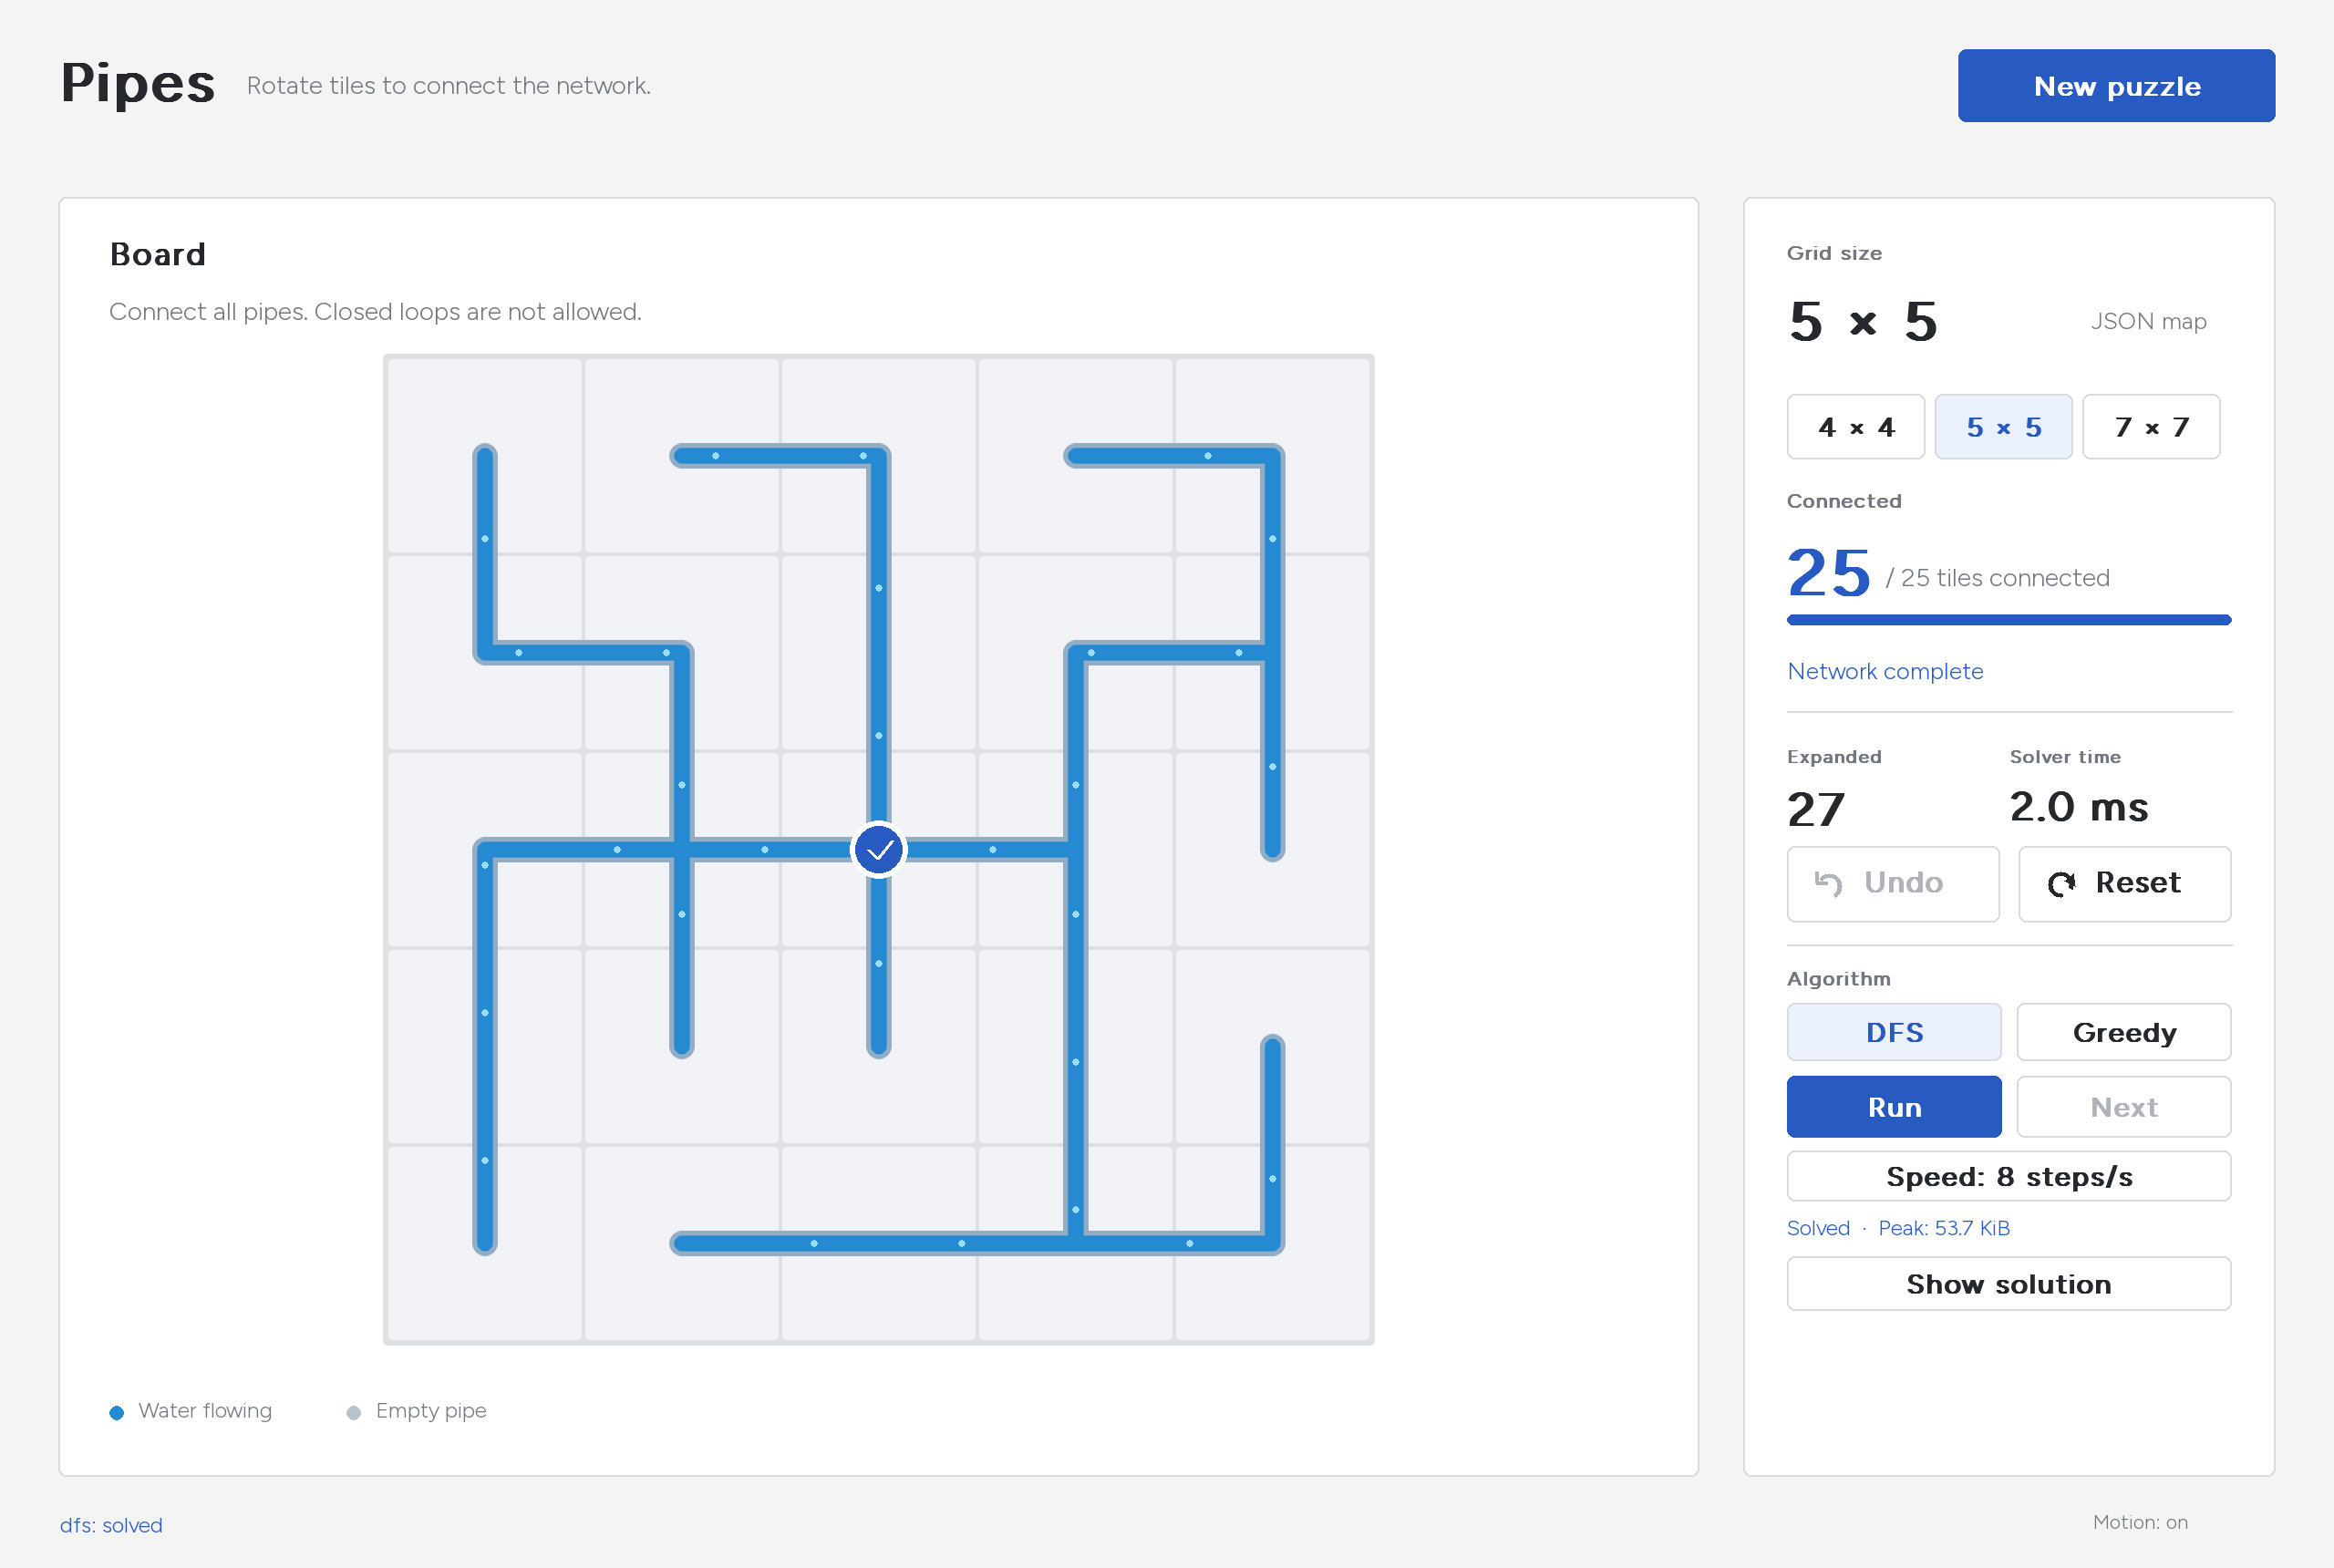
\includegraphics[width=.90\textwidth]{assets/pipes-ui.png}
\caption{Giao diện thực tế: mạng ống chứa nước xanh, điều khiển tìm kiếm và số liệu sau khi giải.}
\label{fig:ui}
\end{figure}

Run bắt đầu từ hướng gốc lưu trong tệp, không sử dụng khóa hay các lần xoay
thủ công trước đó. Pause/Resume và Next cho phép dừng hoặc xem một sự kiện;
Speed đổi tốc độ phát. Show solution phát lại cấu hình trả về tách khỏi quá
trình khám phá. Đổi đầu vào, Reset hoặc đổi thuật toán sẽ hủy phiên hiện tại
và dừng tiến trình đo do phiên đó tạo.

\begin{table}[H]\centering\small
\begin{tabularx}{\textwidth}{@{}lX@{}}\toprule
Sự kiện & Ý nghĩa khi minh họa \\\midrule
\code{expand} & DFS thăm hoặc GBFS lấy một tiền tố từ heap.\\
\code{assign}/\code{queue} & DFS chọn nhánh con hoặc GBFS đưa nhánh con vào heap.\\
\code{reject} & Loại hướng ống vi phạm kiểm tra, kèm viền đỏ và lý do.\\
\code{backtrack} & DFS trở lại tiền tố cha để thử hướng khác.\\\bottomrule
\end{tabularx}
\caption{Sự kiện minh họa không đồng nhất với số trạng thái mở rộng.}
\end{table}

Với \code{pipes-4x4-261.json}, tám sự kiện đầu của DFS là: expand gốc;
assign E cho ô 0; expand $(E)$; reject ES cho ô 1 do thiếu cổng Tây;
assign SW cho ô 1; expand $(E,SW)$; assign E cho ô 2; expand $(E,SW,E)$.
Như vậy, tám sự kiện chỉ tương ứng bốn lần mở rộng.

\section{Đánh giá thực nghiệm}
\subsection{Thiết kế thí nghiệm và phạm vi phép đo}

Các số liệu sử dụng lô thực nghiệm ngày \textbf{22/10/2026}, được lưu cùng mã
nguồn trong thư mục \code{docs/benchmarks/}. Lô gồm chín bản đồ được sinh từ
mạng cây rồi xáo hướng: ba bản đồ cho mỗi cỡ $4\times4$, $5\times5$ và
$7\times7$. Cả hai thuật toán nhận đúng cùng dữ liệu lưu, cùng thứ tự ô,
cùng cắt tỉa và cùng giới hạn: 30 giây tính toán, tối đa 200.000 lần mở rộng.
Mỗi cặp đầu vào và thuật toán chạy năm lần, tổng cộng $9\times2\times5=90$
lượt chạy có đo thời gian.

Môi trường đo là Python 3.13.15, pygame-ce 2.5.8, macOS 26.6.2 trên kiến trúc
ARM64. Các đầu vào là ví dụ tự sinh theo luật tham khảo, không phải các mã
puzzle được chép từ website. Có ba đầu vào độc lập mỗi cỡ; năm lần lặp dùng
đo biến động thực thi, không được xem thành năm bài toán khác nhau.

\begin{enumerate}
\item \textbf{Thời gian.} Dùng \code{time.perf_counter()}~\cite{pytime} cho một
      lượt giải headless, có khởi tạo bộ giải và kiểm tra lời giải cuối, không
      gồm nạp/sinh bản đồ, dựng giao diện, animation hay chờ Next/Pause.
      Giá trị này là thời gian trôi qua của đoạn tính toán, không phải CPU time.
\item \textbf{Bộ nhớ.} Chạy lại trong một lượt riêng với
      \code{tracemalloc}~\cite{pytrace}, lấy đỉnh dung lượng các khối Python
      đang được truy vết tại một thời điểm, đơn vị KiB
      ($1\,\mathrm{KiB}=1024$ byte). Không dùng nó để suy ra
      toàn bộ RSS của tiến trình hay kích thước bộ nhớ của cửa sổ Pygame.
\item \textbf{Ghép phép đo.} Lượt bộ nhớ phải khớp trạng thái kết thúc, lời
      giải trả về và số lần mở rộng với lượt thời gian. Khi không khớp, bộ
      nhớ để trống. Lượt replay dùng cùng ngân sách mở rộng và bỏ giới hạn
      thời gian để overhead đo bộ nhớ không đổi kết quả vì timeout.
\end{enumerate}

Các bảng dùng \textbf{trung vị} thay vì trung bình để giảm ảnh hưởng của một
lần thực thi chậm bất thường. Với bảng theo bản đồ, trung vị lấy trên 5 lần;
với bảng theo cỡ, lấy trên toàn bộ 15 lần thành công của mỗi thuật toán ở cỡ
đó. Thống kê theo cỡ tính trực tiếp trên 15 quan sát, không lấy trung vị của
ba trung vị theo bản đồ. Các bảng được sinh từ CSV gốc đã lưu, với thời gian
được ghi đến 4 chữ số thập phân theo đơn vị ms. Sai khác do làm tròn ở chữ số
cuối không ảnh hưởng kết luận so sánh.

\subsection{Kết quả thực nghiệm của DFS}
% Generated by report/build_tables.py from the published CSV/manifest.

\begin{table}[H]\centering\small
\begin{tabular}{@{}lrrrr@{}}\toprule
Bản đồ & $n$ & Thời gian (ms) & Đỉnh (KiB) & Mở rộng\\\midrule
4x4-261 & 16 & 0.6111 & 26.836 & 17 \\
4x4-262 & 16 & 0.7386 & 27.078 & 21 \\
4x4-263 & 16 & 0.6847 & 26.984 & 17 \\
5x5-261 & 25 & 1.5918 & 53.203 & 27 \\
5x5-262 & 25 & 1.4227 & 53.344 & 26 \\
5x5-263 & 25 & 1.5229 & 53.297 & 26 \\
7x7-261 & 49 & 6.5820 & 145.852 & 55 \\
7x7-262 & 49 & 6.3574 & 145.930 & 53 \\
7x7-263 & 49 & 10.6896 & 145.852 & 82 \\
\bottomrule\end{tabular}
\caption{DFS: trung vị theo từng bản đồ trên 5 lượt thành công. Tên rút gọn 4x4-261 tương ứng pipes-4x4-261.json.}
\end{table}


DFS giải thành công cả 45/45 lượt của bộ chín bản đồ. Với các input này,
số nút mở rộng gần độ sâu lời giải: trường hợp chỉ cần một đường đi hoàn
toàn không quay lui vẫn cần $n+1$ lần mở rộng, bao gồm gốc và đích. Điều này
giải thích con số 17 trên hai input $4\times4$ và 26 trên hai input $5\times5$.
Bản đồ $7\times7$ có hậu tố 263 cần 82 lần mở rộng, cao hơn mức tối thiểu 50,
nhưng vẫn rất nhỏ so với cận toàn bộ không gian cấu hình.

\subsection{Kết quả thực nghiệm của Greedy Best-First Search}
% Generated by report/build_tables.py from the published CSV/manifest.

\begin{table}[H]\centering\small
\begin{tabular}{@{}lrrrr@{}}\toprule
Bản đồ & $n$ & Thời gian (ms) & Đỉnh (KiB) & Mở rộng\\\midrule
4x4-261 & 16 & 0.6931 & 11.695 & 17 \\
4x4-262 & 16 & 0.7990 & 12.359 & 21 \\
4x4-263 & 16 & 0.7755 & 12.500 & 17 \\
5x5-261 & 25 & 1.6749 & 19.500 & 27 \\
5x5-262 & 25 & 1.7578 & 19.219 & 27 \\
5x5-263 & 25 & 1.6577 & 19.219 & 26 \\
7x7-261 & 49 & 8.2135 & 27.594 & 56 \\
7x7-262 & 49 & 7.8395 & 27.070 & 55 \\
7x7-263 & 49 & 12.0140 & 29.094 & 83 \\
\bottomrule\end{tabular}
\caption{GBFS: trung vị theo từng bản đồ trên 5 lượt thành công. Tên rút gọn 4x4-261 tương ứng pipes-4x4-261.json.}
\end{table}


GBFS cũng giải thành công 45/45 lượt. Trên bộ input này, số lần mở rộng bằng
hoặc cao hơn DFS; ví dụ các bản đồ $7\times7$ lần lượt có 56, 55 và 83 lần,
so với 55, 53 và 82 của DFS. Heuristic chưa giảm số trạng thái được mở rộng
trên các input đang xét. Không thể suy ra nó luôn kém hơn trên những input
khác chỉ từ quan sát này.

\Needspace{12\baselineskip}
\subsection{So sánh thời gian, bộ nhớ và mức độ hiệu quả}
% Generated by report/build_tables.py from the published CSV/manifest.

\begin{table}[H]\centering\small
\begin{tabular}{@{}lrrrrr@{}}\toprule
 & \multicolumn{2}{c}{Thời gian (ms)} & GBFS/DFS & \multicolumn{2}{c}{Đỉnh (KiB)}\\
Cỡ & DFS & GBFS & thời gian & DFS & GBFS\\\midrule
$4\times4$ & 0.685 & 0.776 & 1.13 & 26.984 & 12.359 \\
$5\times5$ & 1.518 & 1.692 & 1.12 & 53.297 & 19.219 \\
$7\times7$ & 6.603 & 8.214 & 1.24 & 145.852 & 27.594 \\
\bottomrule\end{tabular}
\caption{Trung vị trên 15 lượt thành công mỗi cỡ và thuật toán. Tỷ lệ lớn hơn 1 nghĩa là GBFS chậm hơn DFS.}
\end{table}


\begin{figure}[H]\centering
% Generated by report/build_tables.py from the published CSV/manifest.

\begin{tikzpicture}
\begin{axis}[width=.48\textwidth,height=5.8cm,ybar,bar width=10pt,
enlarge x limits=.25,ymin=0,xtick={4,5,7},
xticklabels={$4\times4$,$5\times5$,$7\times7$},
ylabel={Thời gian (ms)},
tick label style={font=\footnotesize},label style={font=\small},
ymajorgrids=true,grid style={black!10},
legend style={at={(.5,-.18)},anchor=north,legend columns=2,
draw=none,font=\footnotesize}]
\addplot[fill=pipeblue!75,draw=none,area legend] coordinates {(4,0.6847) (5,1.5177) (7,6.6033)};
\addplot[fill=black!40,draw=none,area legend] coordinates {(4,0.7755) (5,1.6923) (7,8.2135)};
\legend{DFS,GBFS}
\end{axis}\end{tikzpicture}
\hfill
\begin{tikzpicture}
\begin{axis}[width=.48\textwidth,height=5.8cm,ybar,bar width=10pt,
enlarge x limits=.25,ymin=0,xtick={4,5,7},
xticklabels={$4\times4$,$5\times5$,$7\times7$},
ylabel={Đỉnh cấp phát (KiB)},
tick label style={font=\footnotesize},label style={font=\small},
ymajorgrids=true,grid style={black!10},
legend style={at={(.5,-.18)},anchor=north,legend columns=2,
draw=none,font=\footnotesize}]
\addplot[fill=pipeblue!75,draw=none,area legend] coordinates {(4,26.984) (5,53.297) (7,145.852)};
\addplot[fill=black!40,draw=none,area legend] coordinates {(4,12.359) (5,19.219) (7,27.594)};
\legend{DFS,GBFS}
\end{axis}\end{tikzpicture}

\caption{Trung vị thời gian và bộ nhớ đỉnh theo kích thước. Mỗi cột dựa trên
15 lượt thành công của ba bản đồ; dữ liệu là lô ngày 22/10/2026.}
\label{fig:charts}
\end{figure}

\subsubsection{Thời gian thực thi}

Trong bộ đo hiện tại, trung vị thời gian GBFS cao hơn DFS ở cả ba cỡ. Tỷ lệ
GBFS/DFS xấp xỉ 1,13; 1,12 và 1,24 tương ứng $4\times4$, $5\times5$ và
$7\times7$. Hai thuật toán đã dùng cắt tỉa giống nhau và các bản đồ còn ít
nhánh thực sự phải thăm. Trong điều kiện đó, tính điểm $h$, tạo khóa ưu tiên
và thao tác heap có thể tốn nhiều hơn phần công việc tiết kiệm được. Đây là
lời giải thích phù hợp với số mở rộng quan sát được, không phải chứng minh
nhân quả từ một thí nghiệm loại bỏ từng thành phần.

\subsubsection{Không gian lưu trữ}

Bộ nhớ đỉnh được truy vết của DFS lớn hơn GBFS trên bộ dữ liệu này. Đặc điểm
hiện thực góp phần giải thích: DFS giữ các generator đệ quy, các tiền tố tuple
và miền tạm của nhiều mức trong khi đi sâu. GBFS không giữ toàn bộ chuỗi khung
đệ quy đó; với hàng đợi còn nhỏ, phần giữ lại có thể thấp hơn. Kết quả thực
nghiệm không mâu thuẫn với cận xấu nhất của GBFS: nếu nhiều nhánh cùng được
giữ trong heap, bộ nhớ vẫn có thể bùng nổ theo hàm mũ.

\subsubsection{Giới hạn của kết luận thực nghiệm}

Cả hai thuật toán đạt 100\% lượt giải thành công trên lô này, nhưng chỉ có
chín bản đồ tự sinh. Tỷ lệ này chỉ mô tả tập đầu vào đã đo, chưa đủ để suy
rộng mức độ thành công hoặc ưu thế của heuristic trên mọi bài toán Pipes.
Các thời gian nhỏ hơn một mili giây cũng
chịu ảnh hưởng của bộ cấp phát, cache, tải nền và thứ tự chạy trong cùng tiến
trình. Dữ liệu không xác định được một quy luật tăng trưởng tiệm cận từ ba
cỡ lưới. Cần thêm input khó, input vô nghiệm và phép đánh giá bỏ từng lớp
cắt tỉa để đưa ra kết luận tổng quát hơn.

\subsection{Kiểm thử tính đúng đắn và trường hợp vô nghiệm}

Bộ kiểm thử hiện tại có 33 kiểm thử, bao gồm phép xoay và đối xứng, điều kiện
đích, lời giải hợp lệ khác đáp án bộ sinh, việc bỏ qua đáp án ẩn của bộ sinh,
khả thi của tiền tố lời giải đã biết, JSON, giới hạn, hủy phiên, phát lại và
ghi CSV. Cả 33 kiểm thử đều đạt khi rà soát báo cáo ngày 31/10/2026. Các
kiểm thử là bằng chứng kiểm tra hiện thực, không thay thế chứng minh đầy đủ
hay đánh giá trên một tập input lớn.

Bản đồ tùy chỉnh \code{maps/custom/cdai.json} là lưới $4\times4$ gồm 16 ô
một cổng, có tổng 16 cổng. Mạng cây trên 16 ô phải có $2(16-1)=30$ cổng,
nên bản đồ này chắc chắn vô nghiệm, bất kể cách xoay. Cả DFS và GBFS xác nhận
\code{unsolvable} ngay ở gốc, với 0 lần mở rộng. Kiểm tra này được thực hiện
riêng, không được cộng vào 90 lượt benchmark ở trên.

Khi kiểm tra gốc hoặc duyệt hết cây chứng minh không thể hoàn tất, giao diện
hiện thông báo vô nghiệm. Ngược lại, hết 30 giây hoặc 200.000 lần mở rộng
cho kết quả \code{limit_reached}; người dùng dừng phiên cho kết quả
\code{cancelled}. Các trạng thái đó không phải bằng chứng vô nghiệm.

\section{Kết luận cho bài toán Pipes}

Pipes đã được mô hình hóa thành tìm kiếm trên cây gán hướng hữu hạn, với biểu
diễn gọn, tập hành động rõ ràng và bộ kiểm tra đích độc lập. DFS minh họa
chiến lược đi sâu và quay lui; GBFS minh họa chọn trạng thái bằng heuristic
và hàng đợi ưu tiên. Các bước kiểm tra chung bảo đảm việc so sánh không bị
lẫn với thay đổi thứ tự biến hoặc thay đổi luật chơi.

Trên chín đầu vào tự sinh, cả hai giải được mọi lượt chạy; DFS có trung vị
thời gian thấp hơn, còn GBFS có đỉnh cấp phát Python thấp hơn. Heuristic
không làm giảm số trạng thái mở rộng ở bộ đo này, nên không có cơ sở tuyên
bố nó vượt trội tổng quát. Kết quả cần được trình bày cùng điều kiện đo và
giới hạn dữ liệu.

Các hướng phát triển gồm bổ sung tập input khó và có nguồn gốc tham khảo rõ
ràng, thử thứ tự biến hoặc heuristic khác bằng thí nghiệm có kiểm soát, đo
riêng tác động của cắt tỉa, và nghiên cứu bài toán tối thiểu số lần xoay bằng
một mô hình chi phí phù hợp. Những mở rộng này giúp đánh giá rõ hơn tác động
của mô hình trạng thái, ràng buộc và chiến lược duyệt đối với hiệu quả tìm kiếm.
